\documentclass[10pt,a4paper]{article}
\usepackage[textwidth=16cm,textheight=23cm]{geometry}
\usepackage[utf8]{inputenc}
\usepackage[T1]{fontenc}
\usepackage{amsmath}
\usepackage{amsfonts}
\usepackage{amssymb}
\usepackage{graphicx}
%\usepackage{url}
\usepackage{hyperref}
\usepackage{bm}


\newcommand{\Trans}{\mathcal{T}}
\newcommand{\filterationF}{\mathcal{F}}
\newcommand{\mkt}{\mathrm{mkt}}
\newcommand{\ytw}{\mathrm{ytw}}
\newcommand{\dd}{\mathrm{d}}
\newcommand{\CRdelta}{\mathrm{CR01}}

\newcommand{\inVaR}{{\mathrm{iv}}}
\newcommand{\notInVaR}{{\mathrm{niv}}}


\usepackage{tcolorbox}
\tcbuselibrary{theorems}

\newtcbtheorem[number within=section]{MyRemark}{Remark}%
{colback=green!5,colframe=green!35!black,fonttitle=\bfseries}{th}


\parindent=0pt
\parskip=1.5ex


\begin{document}

\title{Note on Deal Contingent Trades}
\author{Youngsuk Lee}
\date{26 July 2020}
\maketitle

\section{Structure}

The firm enters a derivative trade such as FX forwards or FX options with a counterparty where the trade is contingent on an agreed deal such as merger, regulatory approval, etc. 

Consider such a deal-contingent trade (DCT) and its hedge trade, both of which are booked in the trading book. Figure 
\ref{fig:dct-illustration} illustrates two situations:
\begin{itemize}
	\item Deal succeeds where DCT is well hedged throughout its life.  
	\item Deal fails where there is a potential sudden P\&L due to (i) the mark-to-market is {\em released} from DCT and 
	the PV changes from the {\em naked} hedge. 
\end{itemize}

\begin{figure}[h!]
	\begin{center}
		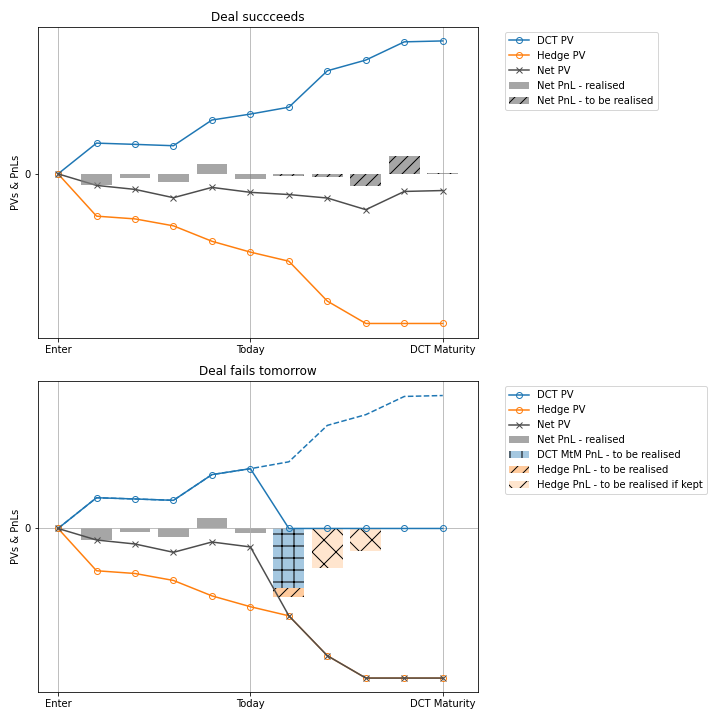
\includegraphics[width=16cm]{figs/dct-illustration.png}
	\end{center}
	\caption{If we put them into the reg VaR and realise the P\&Ls. 
%		left: The deal succeeds. right: The deal fails tomorrow. There are two sources of P\&Ls: (i) blue bar with '+': The mark-to-market of DCT drops to zero.
%		(ii) orange bar with '/': The mark-to-market of the hedge trade moves. 
	}
	\label{fig:dct-illustration}	
	\hrule
\end{figure}

\begin{figure}[h!]
	\begin{center}
		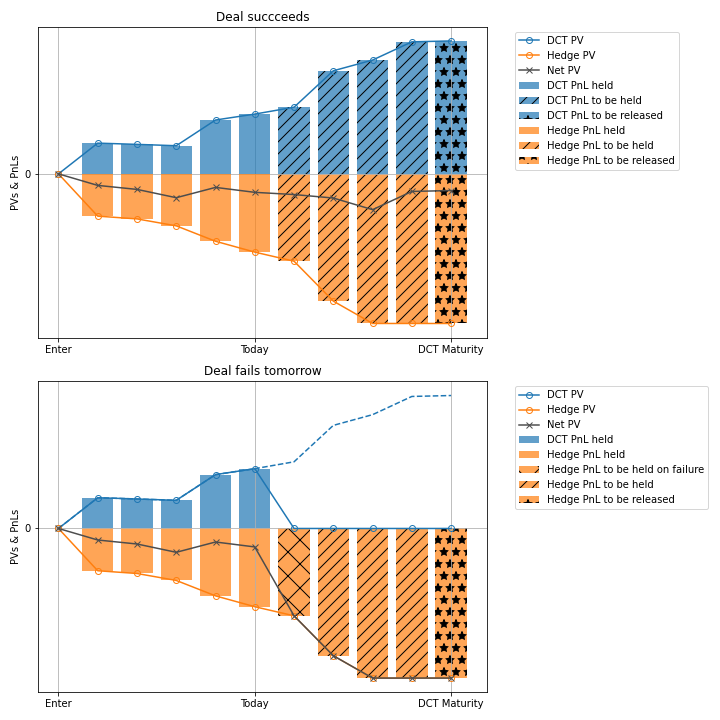
\includegraphics[width=16cm]{figs/dct-illustration-held.png}
	\end{center}
	\caption{
If we put them outside the reg VaR and hold the P\&Ls.. 
	}
	\label{fig:dct-illustration-held}	
	\hrule
\end{figure}

\section{Risk-Not-In-VaR}

\subsection{Risk-Not-In-VaR P\&L}

For typical VaR models, it is not easy to incorporate the risk of deal failures. 

To express the P\&L of this missing risk, let
\begin{itemize}
	\item $V$: mark-to-market of DCT
	\item $\bar{V}$: today's mark-to-market
	\item $\Delta V$: random variable to represent the total P\&L in $V$
	\item $\Delta V^\inVaR$: the part of $\Delta V$ included in VaR. 
	
	For example, if DCT is a simple FX forward on the spot rate $z$, 
	\begin{equation}
	\Delta V^\inVaR = \delta_z \cdot \Delta Z
	\label{eqn:pnl-in-var-example}
	\end{equation}
	where $\delta_z$ is the first-order sensitivity and $\Delta Z$ is the random variable representing the change in $z$. 
	\item $\Delta V^\notInVaR$: the part of $\Delta V$ not included in VaR 
	\item $F$ is the random variable indicating the deal failure:
	\begin{equation}
	F = \left\{ 
	\begin{array}{cl}
		1, & \textrm{if the deal has failed.}\\
		\\
		0, & \textrm{otherwise}
	\end{array}
	\right.
	\end{equation}
\end{itemize}
Then, we have
\begin{equation}
\Delta V = -\bar{V} \cdot F + \Delta V^\inVaR \cdot (1 - F)
\end{equation}
and
\begin{eqnarray}
\Delta V^\notInVaR &=& \Delta V - \Delta V^\inVaR\\
& = & -\bar{V} \cdot F - \Delta V^\inVaR  \cdot F 
\end{eqnarray}

With multiple deals, each of which denoted by $i$, 
\begin{equation}
\Delta V^\notInVaR = \sum_{i=1}^{I}\left[ - \bar{V}_i \cdot F_i
- \Delta V_i^\inVaR \cdot F_i \right]
\label{eqn:missing-pnl}
\end{equation}

\subsection{Model}

To move Eq (\ref{eqn:missing-pnl}), we use a simple multi-variate normal distribution.

\subsubsection{Failure Indicator}
To model $F_i$, we can use a standard framework used for credit default modelling. 

Let $P_i$ be the probability of the deal failure. To simulate the deal failure events, let $X_i$ be an $N(0,1)$ random variable, indicating the deal quality and set
\begin{equation}
F_i := \left\{
\begin{array}{cl}
1, & \textrm{if}\quad \Phi(X_i) < P_i,\\
\\
0, & \textrm{otherwise} 
\end{array}
\right.
\end{equation}

For joint simulations of $\{F_i\}_{i=1}^{I}$, the correlation should be specified:
\begin{equation} 
\rho^F_{i,j} := \mathrm{corr}(F_i, F_j).
\end{equation}



\subsubsection{VaR P\&Ls}

To model $\Delta V_i^\inVaR$, without loss of generality, assume that it can be written as a function of $\Delta \bm{Z}$, the return distribution of a set of risk factors $\bm{z} = [z_1, \cdots, z_K]$ included in VaR:
\begin{equation}
\Delta V_i^\inVaR := \Delta V_i^\inVaR(\Delta \bm{Z})
\end{equation}
As an example, see Eq (\ref{eqn:pnl-in-var-example}). 

\begin{MyRemark}{VaR P\&L functions}{}
$\Delta V_i^\inVaR$ is the same P\&L (approximation) function used in VaR.
\end{MyRemark}

We assume that $\Delta Z$ follows a multi-variate normal distribution with
\begin{equation}
\Delta Z_k \sim N(\mu_k, \sigma_k^2) \quad \textrm{and} \quad \mathrm{corr}(\Delta Z_k, \Delta Z_l) = \rho_{k,l}^{Z}.
\end{equation}

\subsubsection{Correlation: Deal Failures and Risk Factors}

Finally, the correlations among deal quality indices $X_i$'s and VaR risk factors $Z_k$'s should be specified:
\begin{equation}
\rho_{i,k}^{F,Z} = \mathrm{corr}(X_i, Z_k)
\end{equation}



\subsection{Model Parameter Estimations}

{\bf Postulations}: The following parameters are postulated by appropriate {\em experts}:
\begin{itemize}
	\item Failure Probability and Correlations: 	$\{P_i\}$ and $\{\rho^F_{i,j}\}$ where $i, j = 1, \cdots, I$
	\item Deal vs market correlations: $\{ \rho_{i,k}^{F,Z}\}$ for $i = 1, \cdots, I$ and $k = 1, \cdots, K$. 
	
	Due to the nature of typical deal contingent trades, they would be set to zero. 
	
\end{itemize}


{\bf Calibrations}: The following risk factor model parameters 
\begin{center}
	$\{\mu_k\}$, $\{\sigma_k\}$ and $\{\rho_{k,l}^Z\}$ where $k, l = 1, \cdots, I$: 
\end{center}
would be calibrated to simulated returns of the relevant historical VaR models. 

\subsection{Quantification}

\begin{enumerate}
	\item Run standard Monte Carlo simulations on 
	\begin{equation}
	\{X_i\}_{i=1}^{I}\quad\textrm{and}\quad\{Z_k\}_{k=1}^{K}.
	\end{equation}
	\item Generate scenarios of the risk-not-in-VaR P\&L $\Delta V^\notInVaR$ using Eq (\ref{eqn:missing-pnl}).
	\item Calculate the 99th tail measure.
\end{enumerate}

\end{document}